\documentclass{beamer}
\mode<presentation>
  {
%   \usetheme{Berlin}
  %\usetheme{Dreuw}
  \usetheme{Dreuw}
  }
%  \usepackage{times}
  \usepackage{subfigure}
  \usepackage{relsize}
  \usepackage{tikz}
  \usepackage{amsmath,amsthm, amssymb, latexsym}
 % \boldmath
  \renewcommand*{\thesubfigure}{}
%  \renewcommand{\figurename}{bvla}

\makeatletter
\providecommand\dotsum{\mathpalette\@dotted\sum \vphantom{\sum}}
\def\@dotted#1#2{\ooalign{\hfil$#1 \bullet $\hfil\cr\hfil$#1#2$\hfil\cr}}
\makeatother
\DeclareMathOperator*{\psum}{\mathchoice{\sum\!\!\!\!\!\!\!\bullet\ \ }{\sum\hspace{-2.2ex}\raisebox{0.2ex}{\scalebox{0.75}{$\bullet$}}\,\,}{\sum\!\!\!\!\!\!\!\bullet}{\sum\!\!\!\!\!\!\!\bullet}}
\DeclareMathOperator*{\psumm}{\mathchoice{\sum\!\!\!\!\!\!\!\bullet\ \ }{\sum\hspace{-2.6ex}\raisebox{0.15ex}{\scalebox{0.75}{$\bullet$}}\,\,}{\sum\!\!\!\!\!\!\!\bullet}{\sum\!\!\!\!\!\!\!\bullet}}

\DeclareMathOperator*{\pplus}{\oplus}
\newcommand{\dv}{\vec{t}}

  \usetikzlibrary{backgrounds}
\usetikzlibrary{automata}
\usetikzlibrary{arrows}
\usetikzlibrary{shapes}
\usetikzlibrary{decorations.pathmorphing}
\usetikzlibrary{fit}

\let\picturesize\Large

\def\clap#1{\hbox to 0pt{\hss#1\hss}}
\def\mathclap{\mathpalette\mathclapinternal}
\def\mathllap{\mathpalette\mathllapinternal}
\def\mathrlap{\mathpalette\mathrlapinternal}
\def\mathclapinternal#1#2{%
            \clap{$\mathsurround=0pt#1{#2}$}}
\def\mathllapinternal#1#2{%
            \llap{$\mathsurround=0pt#1{#2}$}}
\def\mathrlapinternal#1#2{%
            \rlap{$\mathsurround=0pt#1{#2}$}}


%%%%% TIKZ
\tikzstyle{every picture}=[line width=4pt]
\tikzstyle{ultra ultra thick}=[line width=2.5pt]
\tikzstyle{nodeSmall} = [state, minimum size=6mm, inner sep=0mm, fill=black, node distance=1.25cm]
\tikzstyle{state2}=[state, minimum size=7mm, inner sep=0.5mm]
\tikzstyle{teststate}=[state, minimum size=4mm, inner sep=0.5mm]
\tikzstyle{testleaf}=[minimum size=4mm, inner sep=0.5mm]
\tikzstyle{every loop}=[->]
\tikzstyle{onEdge}=[fill=white, pos=0.4]
\tikzstyle{testschuin}=[node distance=\testschuin]
\tikzstyle{test}=[node distance=\test, pos=0.4]
\tikzstyle{loopupper}=[in=67, out=113, loop]
\tikzstyle{lagerLabel}=[pos=0.68]
\tikzstyle{every scope}=[>=latex, node distance=\recht]
\tikzstyle{smallstate}=[state, minimum size=3mm, inner sep=0.5mm, fill=white, ultra ultra thick]
\tikzstyle{smallstate3}=[state, minimum size=3mm, inner sep=2mm, fill=white]
\tikzstyle{smallrectangle}=[state, rectangle, minimum size=3mm, inner sep=0.5cm, fill=white]
\tikzstyle{smallstate2}=[state, minimum size=5mm, inner sep=0.5mm, fill=white]
\tikzstyle{background rectangle}= [rounded corners, fill=yellow!20, draw=black, rounded corners=1ex]
\tikzstyle{oval} = [state, ellipse, minimum size=4mm, inner sep=0.5mm, node distance=1.5cm]
\tikzstyle{prob}=[->, decorate, decoration={snake,segment length=2mm, amplitude=.4mm,post length=1mm}]




\tikzstyle{loopleft}=[in=-176, out=-184, loop, swap]
\definecolor{greenish}{rgb}{0,0.5,0}
\tikzstyle{loopright}=[in=-10, out=10, loop, swap]
\tikzstyle{loopleft2}=[in=-171, out=-189, loop, swap]

\newlength{\testschuin}
\newlength{\test}
\newlength{\recht}
\setlength{\testschuin}{2.1213203435596425732025330863145cm}
\setlength{\test}{1.5cm}
\setlength{\recht}{1.7677669529663688110021109052621cm}
\newcommand{\back}{\picturesize \color{yellow!20}.}
\newcommand{\fail}{\bf \vphantom{p}fail\vphantom{f}}
\newcommand{\pass}{\bf \vphantom{p}pass\vphantom{f}}
%%%%%%%% TIKZ


  \usepackage[english]{babel}
  \usepackage[latin1]{inputenc}
%   \usepackage[textpos}
  \usepackage[absolute,overlay]{textpos}
  \usepackage[orientation=portrait,size=a0,scale=1.35,debug]{beamerposter}

  %%%%%%%%%%%%%%%%%%%%%%%%%%%%%%%%%%%%%%%%%%%%%%%%%%%%%%%%%%%%%%%%%%%%%%%%%%%%%%%%%5
  \graphicspath{{figures/}}

  \title[]{\Huge Probabilistic specifications with data types}
  \author[]{\LARGE \textbf{Joost-Pieter Katoen, Jaco van de Pol, Mari\"elle Stoelinga, Mark Timmer}}

  \institute{\Large \vfill {Formal Methods and Tools -- Department of Computer Science -- University of Twente} }
  \date{November 5, 2009}

  \begin{document}
  \begin{frame}{}

\vspace{-1cm}
% Eerste rij
\begin{columns}[t]
\begin{column}{.02\linewidth}\end{column}
\begin{column}{.97\linewidth}\setbeamertemplate{block begin}{
  \vskip.75ex
  \begin{beamercolorbox}[rounded=true,shadow=true,leftskip=1cm,colsep*=.75ex]{block title}%
    \usebeamerfont*{block title}\insertblocktitle
  \end{beamercolorbox}%
  {\ifbeamercolorempty[bg]{block body}{}{\nointerlineskip\vskip-0.5pt}}%
  \usebeamerfont{block body}%
  \begin{beamercolorbox}[rounded=true,shadow=true,colsep*=.75ex,sep=.75ex, vmode]{block body}%
    \ifbeamercolorempty[bg]{block body}{\vskip-.25ex}{\vskip-.75ex}\vbox{}%
    \begin{adjustwidth}{0.8cm}{0.4cm}
  }
  \setbeamertemplate{block end}{
  \end{adjustwidth}
  \end{beamercolorbox}
}


\begin{block}{\large \smash{1. Introduction}\vphantom{Introduction}}

\begin{columns}[T]
\begin{column}{0.01\linewidth}\end{column}
\begin{column}{.48\linewidth}
\alert{Dependability} of computer systems is becoming more and more important.

\ 

\begin{figure}[h!]
\hfill
\subfigure[Windows blue screen]{
\newcommand{\bluescreen}[1]{\color{white}\texttt{#1}}

\tikzstyle{background rectangle}= [fill=blue!60!black, draw=white]
\begin{tikzpicture}[scale=1, show background rectangle]
\node[] (s_1) {\scalebox{0.25}{
\begin{minipage}{42cm}
\noindent\\\noindent\\\noindent\\\noindent\\\noindent\\\noindent\\
\noindent{\color{blue!60!black}x}\texttt{\ \ \ \ \ \ \ \ \ \ \ \ \ \ \ \ \ \ \ \ \ \ \ \ \ \ \ \ \ \ }\colorbox{gray}{\color{blue!60!black}\texttt{\phantom{.}Windows\phantom{.}}\vphantom{$\sum_{n=0}^\infty$}}\\\noindent\\
\bluescreen{A fatal exception 0E has occurred at 0137:BFFA21C9. The current}\\
\bluescreen{application will be terminated.}\\
\noindent\\
\bluescreen{* Press any key to terminate the current application.}\\
\bluescreen{* Press CTRL+ALT+DEL again to restart your computer. You will}\\
\bluescreen{\ \ lose any unsaved information in all application.}\\
\noindent\\
\bluescreen{\ \ \ \ \ \ \ \ \ \ \ \ \ \ \ \ \ \ \ \ \ Press any key to continue}
\noindent\\\noindent\\\noindent\\\noindent\\\noindent\\\noindent\\
\end{minipage}
}};
\end{tikzpicture}
}
\hfill
\subfigure[Ariane 5 crash]{
\raisebox{0.08cm}{
%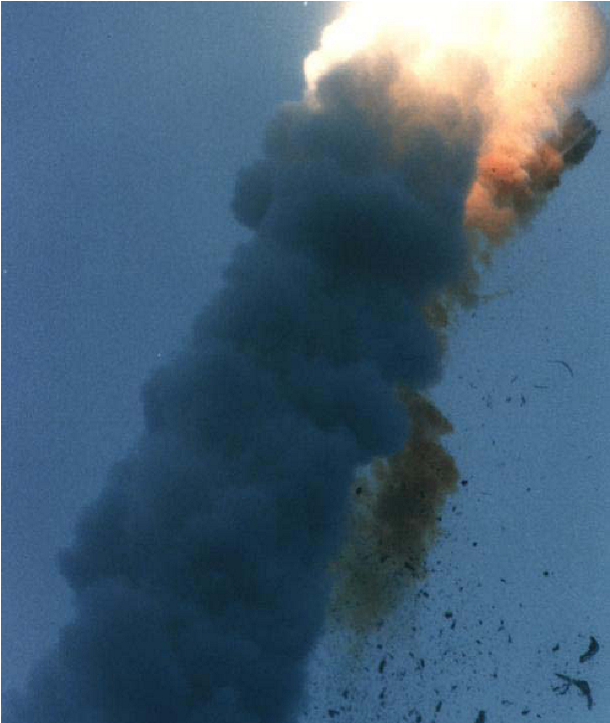
\includegraphics[scale=0.573]{figures/ariane5-2.png}
}}
\hfill
{}
\end{figure}
%%% Eind plaatjes

\noindent \\[65pt]

Our aim is to use \alert{formal methods} to improve system quality.

\end{column}
\begin{column}{.02\linewidth}
\begin{tabular}{cc|}
&\\
&\\
&\\
&\\
&\\
&\\
&\\
&\\
&\\
&\\
&\\
\end{tabular}
\end{column}
\begin{column}{.48\linewidth}
A popular solution is \alert{model checking}; verifying \alert{properties} of a system by constructing a \alert{model} and ranging over its \alert{state space}. \

\vskip-20pt

\begin{columns}
\begin{column}{0.02\linewidth}\end{column}
\begin{column}{.48\linewidth}
\begin{figure}[h!]
\subfigure[An overview of model checking]{
\begin{tikzpicture}[scale=0.7, transform shape] 
\node[] (sinit) {};
\node[cloud, fill=white, draw=black, cloud puffs=15, aspect=2.5, inner sep=0pt, cloud puff arc=120, text=black] (s0) [right of=sinit, node distance=7cm] {\bf $\mathrlap{\text{\ \ \ \ System}}$\phantom{Requirements}}; 
\node[smallrectangle] (s1) [below of=s0, node distance=7cm] {$\mathrlap{\text{\ \:Model}}\phantom{Property}$};
\node[cloud, fill=white, draw=black, cloud puffs=15, aspect=2.5, inner sep=0pt, cloud puff arc=120, text=black] (s2) [right of=s0, node distance=15cm] {\bf Requirements}; 
\node[smallrectangle] (s3) [below of=s2, node distance=7cm] {Property};
\draw[->] (s0) edge (s1);
\draw[->] (s2) edge (s3);
\node[] (temp) [below of=s1, node distance=6cm] {};
\node[smallrectangle] (s4) [right of=temp, node distance=7.5cm] {Model checker};
\draw[->] (s1) edge (s4);
\draw[->] (s3) edge (s4);
\node[oval, inner sep=0.4cm, fill=red] (s5) [left of=s4, node distance=9cm] {Fail};
\node[oval, inner sep=0.4cm, fill=green] (s6) [right of=s4, node distance=9cm] {Pass};
\draw[->] (s4) edge (s5);
\draw[->] (s4) edge (s6);
\draw[->] (s5) edge (s1);

\end{tikzpicture}
}
\end{figure}
\end{column}
\begin{column}{.12\linewidth}\end{column}
\begin{column}{.36\linewidth}
\begin{figure}
\vskip23pt
\subfigure{
\begin{tikzpicture}[scale=1.25, transform shape, show background rectangle, node distance=2.5cm, descr/.style={fill=white,inner sep=2.5pt}]
 
	   \path (0.5,0) node[smallstate, fill=green] (s_0) {}
             (1.5,-1) node [smallstate, fill=green] (s_1) {}
	   (2.1, 0.5) node [smallstate, fill=green] (s_2) {}
	   (2.8, -0.25) node [smallstate, fill=green] (s_3) {}
	   (4, 0.45) node [smallstate, fill=green] (s_4) {}
	   (3.3, -1) node [smallstate, fill=green] (s_5) {}
	   (4.2, -0.8) node [smallstate, fill=green] (s_6) {}
	   (1.1, -2.4) node [smallstate, fill=green] (s_7) {}
	   (2.5, -2.0) node [smallstate, fill=green] (s_8) {}
	   (3.55, -1.75) node [smallstate, fill=green] (s_9) {}
	   (4.5, -2.3) node [smallstate, fill=green] (s_10) {}
	  (2.4, -3) node [smallstate, fill=green] (s_11) {}
	  (3.8, -3.2) node [smallstate, fill=green] (s_12) {};
	   
	   	
	\draw[->, ultra ultra thick ] (s_0) edge (s_1);
	\draw[->, ultra ultra thick] (s_1) edge (s_2);
	\draw[->, ultra ultra thick] (s_1) edge (s_3);
	\draw[->, ultra ultra thick] (s_3) edge (s_4);
	\draw[->, ultra ultra thick] (s_4) edge (s_5);
	\draw[->, ultra ultra thick] (s_4) edge (s_6);
	\draw[->, ultra ultra thick] (s_1) edge (s_7);
	\draw[->, ultra ultra thick] (s_7) edge (s_8);
	\draw[->, ultra ultra thick] (s_8) edge (s_9);
	\draw[->, ultra ultra thick] (s_8) edge (s_11);
	\draw[->, ultra ultra thick] (s_9) edge (s_10);
	\draw[->, ultra ultra thick] (s_10) edge (s_12);
	
\end{tikzpicture}
}
%
\subfigure[\qquad \qquad \qquad \qquad \ $\mathllap{\text{The output of model checking}}$]{
\begin{tikzpicture}[scale=1.25, transform shape, show background rectangle, node distance=2.5cm, descr/.style={fill=white,inner sep=2.5pt}]
      \path
    	(0.5,0) node[smallstate, fill=green] (s_0) {}
             (1.5,-1) node [smallstate, fill=green] (s_1) {}
	   (2.1, 0.5) node [smallstate, fill=green] (s_2) {}
	   (2.8, -0.25) node [smallstate, fill=green] (s_3) {}
	   (4, 0.45) node [smallstate, fill=green] (s_4) {}
	   (3.3, -1) node [smallstate, fill=green] (s_5) {}
	   (4.2, -0.8) node [smallstate, fill=green] (s_6) {}
	   (1.1, -2.4) node [smallstate, fill=green] (s_7) {}
	   (2.5, -2.0) node [smallstate, fill=green] (s_8) {}
	   (3.55, -1.75) node [smallstate, fill=green] (s_9) {}
	   (4.5, -2.3) node [smallstate, fill=green] (s_10) {}
	  (2.4, -3) node [smallstate, fill=red] (s_11) {}
	  (3.8, -3.2) node [smallstate, fill=green] (s_12) {};
	   	
	\draw[->, ultra ultra thick, color=blue, densely dotted] (s_0) edge (s_1);
	\draw[->, ultra ultra thick] (s_1) edge (s_2);
	\draw[->,ultra ultra thick] (s_1) edge (s_3);
	\draw[->,ultra ultra thick] (s_3) edge (s_4);
	\draw[->,ultra ultra thick] (s_4) edge (s_5);
	\draw[->,ultra ultra thick] (s_4) edge (s_6);
	\draw[->, ultra ultra thick, color=blue, densely dotted] (s_1) edge (s_7);
	\draw[->, ultra ultra thick, color=blue, densely dotted] (s_7) edge (s_8);
	\draw[->,ultra ultra thick] (s_8) edge (s_9);
	\draw[->, ultra ultra thick, color=blue, densely dotted] (s_8) edge (s_11);
	\draw[->,ultra ultra thick] (s_9) edge (s_10);
	\draw[->,ultra ultra thick] (s_10) edge (s_12);
		
\end{tikzpicture}
}
\end{figure}

\begin{textblock}{5}(80.5,36.3)
\parbox{5cm}{\raggedleft Pass:}
\end{textblock}
\begin{textblock}{5}(80.5,47.1)
\parbox{5cm}{\raggedleft Fail:}
\end{textblock}


\end{column}
\begin{column}{0.02\linewidth}\end{column}
\end{columns}
\end{column}
\begin{column}{.01\linewidth}\end{column}
\end{columns}
\end{block}	
\end{column}
\begin{column}{.02\linewidth}\end{column}
\end{columns}

\vskip0.01\linewidth
%\vfill

% Tweede rij
\begin{columns}[t]
\begin{column}{.02\linewidth}\end{column}
\begin{column}{.475\linewidth}\begin{block}{\large \smash{Introduction}\vphantom{Introduction}}
\end{block}

\end{column}
\begin{column}{.01\linewidth}\end{column}
\begin{column}{.475\linewidth}\chapter{Overview}
\ac{ESSIG} is roughly composed out of three components. First we have
the input language, which can be used to describe the micro controller a
simulator should be generated for. Than we have a generator, which
creates an implementation of the private API (see VM) that the VM can
use in simulating the micro controller. Than we have our VM, in which
the micro controller will be simulated. It exposes a public API to a
client which can then simulate programs like they were running on the
simulator. The following diagram illustrates how the components relate
to each other.

\begin{center}
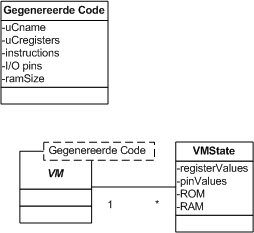
\includegraphics[width=5.376cm,height=4.932cm]{Essig-img002.png}
\end{center}

\end{column}
\begin{column}{.02\linewidth}\end{column}
\end{columns}

%\vfill
\vskip0.01\linewidth

\begin{columns}[t]
\begin{column}{.02\linewidth}\end{column}
\begin{column}{.475\linewidth}\setbeamertemplate{block begin}{
  \vskip.75ex
  \begin{beamercolorbox}[rounded=true,shadow=true,leftskip=1cm,colsep*=.75ex]{block title}%
    \usebeamerfont*{block title}\insertblocktitle
  \end{beamercolorbox}%
  {\ifbeamercolorempty[bg]{block body}{}{\nointerlineskip\vskip-0.5pt}}%
  \usebeamerfont{block body}%
  \begin{beamercolorbox}[rounded=true,shadow=true,colsep*=.75ex,sep=.75ex, vmode]{block body}%
    \ifbeamercolorempty[bg]{block body}{\vskip-.25ex}{\vskip-.75ex}\vbox{}%
    \begin{adjustwidth}{0.8cm}{0.4cm}
  }
  \setbeamertemplate{block end}{
  \end{adjustwidth}
  \end{beamercolorbox}
}

\begin{block}{\large \smash{4. The process algebra prCRL}\vphantom{Introduction}}
We introduce the specification language \alert{prCRL}, give by
\begin{align*}\color{black}
     p ::= Y(\dv) \ \mid\  c \Rightarrow p \ \mid \ p + p \ \mid \ \sum_{x:D} p \ \mid \ a(\dv) \!\!\psum_{x :D} f \colon p
\end{align*}
where $c$ is a \alert{condition}, $a$ an atomic \alert{action}, $f$ a \alert{real-valued expression} yielding values in $[0,1]$, and $\dv$ a \alert{vector of expressions}. 

\vskip20pt

\begin{adjustwidth}{0.5cm}{0.5cm}
\begin{itemize}
\item \ Based on $\mu$CRL (so \alert{data}), with additional \alert{probabilistic choice}
\item \ Operational semantics defined in terms of \alert{probabilistic automata}
\item \ Minimal set of operators to \alert{facilitate formal manipulation}
\item \ \alert{Syntactic sugar} easily definable
\end{itemize}
\end{adjustwidth}

\vskip20pt

\textit{Example:} $X = \tau \psum_{n:\mathbb{N}} \frac{1}{2^n}\colon \text{\it send}(n) \cdot X$. This specification repeatedly chooses a natural number $n$ with probability $\frac{1}{2^n}$, and then sends the number.
\end{block}	
\end{column}
\begin{column}{.01\linewidth}\end{column}
\begin{column}{0.475\linewidth}\setbeamertemplate{block begin}{
  \vskip.75ex
  \begin{beamercolorbox}[rounded=true,shadow=true,leftskip=1cm,colsep*=.75ex]{block title}%
    \usebeamerfont*{block title}\insertblocktitle
  \end{beamercolorbox}%
  {\ifbeamercolorempty[bg]{block body}{}{\nointerlineskip\vskip-0.5pt}}%
  \usebeamerfont{block body}%
  \begin{beamercolorbox}[ht=19.33cm, rounded=true,shadow=true,colsep*=.75ex,sep=.75ex, vmode]{block body}%
    \ifbeamercolorempty[bg]{block body}{\vskip-.25ex}{\vskip-.75ex}\vbox{}%
    \begin{adjustwidth}{0.8cm}{0.4cm}
  }
  \setbeamertemplate{block end}{
  \end{adjustwidth}
  \end{beamercolorbox}
}
\begin{block}{\large \smash{5. The linear format: LPPE}\vphantom{Introduction}}
We define \alert{LPPEs} (linear probabilistic process equations) as follows:
\vskip-25pt
\begin{align*}
X(\vec{g\vphantom{G}}:\vec{G}) = & \sum_{\vec{d_1} : \vec{D_1}} c_1 \Rightarrow a_1(b_1) \!\psum_{\vec{\vphantom{E}e_1} : \vec{E_1}} f_1 \colon X(n_1)\\
& \dots\\[10pt]
 + & \sum_{\vec{d_k} : \vec{D_k}} c_k \Rightarrow a_k(b_k) \!\psum_{\vec{\vphantom{E}e_k} : \vec{E_k}} f_k \colon X(n_k)
\end{align*}

\vskip40pt

Advantages of LPPEs:
\begin{adjustwidth}{0.5cm}{0.5cm}
\begin{itemize}
\item \ The \alert{state space} can be generated very easily
\item \ \alert{Parallel composition} can be applied in a straight-forward manner
\item \ \alert{Symbolic optimisations} are enabled at the language level
\end{itemize}
\end{adjustwidth}
\end{block}	\end{column}
\begin{column}{.02\linewidth}\end{column}
\end{columns}

\vskip0.01\linewidth
%\vfill

% Derde rij
\begin{columns}[t]
\begin{column}{.02\linewidth}\end{column}
\begin{column}{.475\linewidth}\begin{block}{\large \smash{Example Specficication}\vphantom{Example Code}}

\tiny {  
\lstset{
numbers=left,                   % where to put the line-numbers
numberstyle=\tiny,      % the size of the fonts that are used for the line-numbers
stepnumber=1,
xleftmargin=25pt,
backgroundcolor=\color{lightgray},
frame=single
}

Specify the microcontroller as type 'demo'.
\begin{lstlisting}
demo {
\end{lstlisting}

Define general parameters.
\begin{lstlisting}[name=demo.dmo]
	parameters {
		gprs 2+5;
		opcode-size 16;
		clock 1;
		endianness little;
	}
\end{lstlisting}

Define register offsets.
\begin{lstlisting}[name=demo.dmo]
	registers {
		SREG	= 0x5F;
		PC	= 0x462;
		SP	= 0x5D;
	}
\end{lstlisting}

Define memory mappings.
\begin{lstlisting}[name=demo.dmo]
	maps {
		chunk		(0, 0xFFFFFFF);
		register	(0, 0x20);
		io		(0x20, 0x60);
		ram		(0, 0x461);
		rom		(0x464, 0xFFFFFF);
		print		(0x3b, 0x3c);
	}

\end{lstlisting}

Define instructions
\begin{lstlisting}[name=demo.dmo]
	instructions {
		noop "0000 0000 0000 0000" {
			PC = PC + 1;
		}

		/* Load an I/O Location to Register */
		in "1011 0AAd dddd AAAA" Rd, A {
			Rd = io($A);

			PC = PC + 1;
		}

		jmp "1001 010k kkkk 110k", "kkkk kkkk kkkk kkkk" k {
			PC = $k;
		}
	}
}  
\end{lstlisting}

}

\end{block}
\end{column}
\begin{column}{.01\linewidth}\end{column}
\begin{column}{0.475\linewidth}

\setbeamertemplate{block begin}{
  \vskip.75ex
  \begin{beamercolorbox}[rounded=true,shadow=true,leftskip=1cm,colsep*=.75ex]{block title}%
    \usebeamerfont*{block title}\insertblocktitle
  \end{beamercolorbox}%
  {\ifbeamercolorempty[bg]{block body}{}{\nointerlineskip\vskip-0.5pt}}%
  \usebeamerfont{block body}%
  \begin{beamercolorbox}[ht=17.45cm, rounded=true,shadow=true,colsep*=.75ex,sep=.75ex, vmode]{block body}%
    \ifbeamercolorempty[bg]{block body}{\vskip-.25ex}{\vskip-.75ex}\vbox{}%
    \begin{adjustwidth}{0.8cm}{0.4cm}
  }
  \setbeamertemplate{block end}{
  \end{adjustwidth}
  \end{beamercolorbox}
}

\begin{block}{\large \smash{7. Results and Future Work} \vphantom{Introduction}}
\textbf{Results:}
\begin{adjustwidth}{0.5cm}{0.5cm}
\begin{itemize}
\item \ We developed the \alert{process algebra prCRL}, incorporating both \alert{data} and 
\item[] \ \alert{probability}.
\item \ We defined a \alert{linear format for prCRL}, the \alert{LPPE}, providing the starting 
\item[] \ point for effective symbolic optimisations and easy state space generation.
\item \ We provided a \alert{linearisation algorithm} to transform prCRL  specifications 
\item[]\  to their corresponding LPPE, proved it \alert{correct}, and \alert{implemented} it.
\end{itemize}
\end{adjustwidth}

\noindent\\ \phantom{x}\noindent\\

\textbf{Future work:}
\begin{adjustwidth}{0.5cm}{0.5cm}
\begin{itemize}
\item \ Applying existing optimisation techniques, such as \alert{constant elimination},
\item[] \  \alert{liveness analysis} and \alert{confluence reduction}, to LPPEs.
\end{itemize}
\end{adjustwidth}
\vskip10pt
\end{block}

\vskip0.02\linewidth

\setbeamertemplate{block begin}{
  \vskip.75ex
  \begin{beamercolorbox}[rounded=true,shadow=true,leftskip=1cm,colsep*=.75ex]{block title}%
    \usebeamerfont*{block title}\insertblocktitle
  \end{beamercolorbox}%
  {\ifbeamercolorempty[bg]{block body}{}{\nointerlineskip\vskip-0.5pt}}%
  \usebeamerfont{block body}%
  \begin{beamercolorbox}[rounded=true,shadow=true,colsep*=.75ex,sep=.75ex, vmode]{block body}%
    \ifbeamercolorempty[bg]{block body}{\vskip-.25ex}{\vskip-.75ex}\vbox{}%
    \begin{adjustwidth}{0.8cm}{0.4cm}
  }
  \setbeamertemplate{block end}{
  \end{adjustwidth}
  \end{beamercolorbox}
}

%\vskip45pt

\begin{block}{\large \smash{8. Acknowledgments} \vphantom{Introduction}}
This research is supported by NWO under grant 612.063.817 (SYRUP) 
and grant Dn 63-257 (ROCKS), and by the European Union under FP7-ICT-2007-1 
grant 214755 (QUASIMODO).
\end{block}
\end{column}
\begin{column}{.02\linewidth}\end{column}
\end{columns}

%\vfill

\end{frame}
\end{document}
